\chapter{Reconstruction}

A telescope is only as good as it's ability to identify distinct sources. In the case of a neutrino telescope this translates directly to how well observed events can be reconstructed for the direction of high energy events. IceCube uses several reconstruction methods \cite{icecube} and has several data quality checks it must go through before a result is given any weight. Similarly, ANTARES has had years of work put into the reconstruction software in order to reach the accuracies it can now \cite{antares}. To set the context for reconstructions, we need to first understand the data that is collected and how it appears. 

\section{Geometry of a Single Hit}

At first thought, it may sound simple to try and reproduce the tracks that produce the light one would observe in neutrino detectors, but upon considering the data that is aquired the true complexity is revealed. To see this, we consider first the geometry of a single hit to see what the data would look like. Referring to Figure \ref{fig:ghit}, we consider a muon track that is infinite in length, which is a safe approximation assuming a sufficient energy of the neutrino relative to the size of the detector. Specifically we can parameterize the track with
\begin{equation}\label{eq:track}
  \vec{u}(t) = \vec{x} + ct\vec{v}\, ,
\end{equation}
where $\vec{x}$ is the vertex, $\vec{v}$ is the direction the muon is travelling in, $t$ is the time parameter, and finally $c$ is the speed of light, which again for sufficiently high energy muons is a good approximation for the speed. Looking at the $i^{\text{th}}$ DOM located at a position $\vec{r_{i}}$, it is easy to see there must be a closest approach position for the track, $\vec{p}_{i}$, and emission point of a photon given there is a direct hit on the DOM, located at $\vec{q}_{i}$. The photon is emitted at a cherenkov angle of $\theta_{c}$, which is as described in equation \ref{fig:cher_angle}. 


\begin{figure}
  \centering
  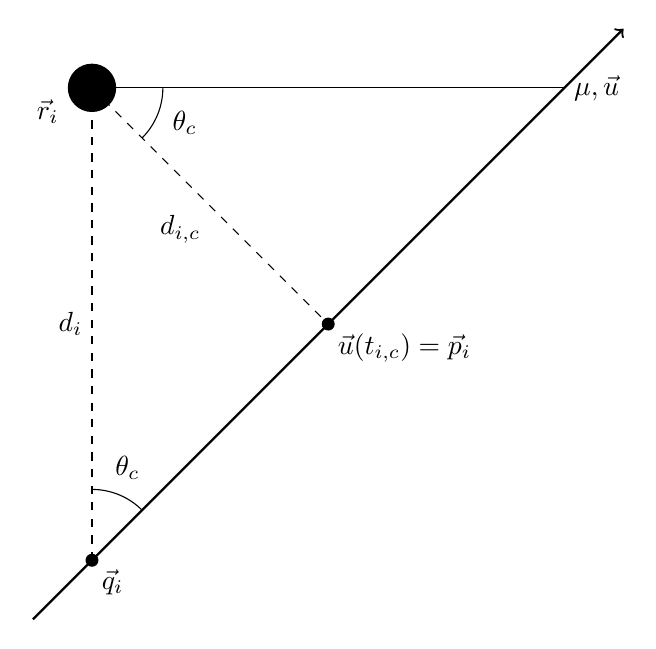
\begin{tikzpicture}[scale=3]
    % Closest point to DOM
    \node [below right] at (0,0) {$\vec{u}(t_{i,c}) = \vec{p}_{i}$};
    \node [below left] at (-0.5, 0.5) {$d_{i,c}$};
    \draw[fill] (0,0) circle [radius=0.025];
    \draw [dashed] (-1,1) -- (0,0);
    % Muon Travel line
    \draw [thick, ->] (-1.25,-1.25) -- (1.25,1.25);
    \node [right] at (1,1) {$\mu, \vec{u}$};
    % Emission point
    \node [below right] at (-1,-1) {$\vec{q}_{i}$};
    \node [above] at (-0.85, -0.7) {$\theta_{c}$};
    \draw[fill] (-1,-1) circle [radius=0.025];
    \draw (-1,-0.7) arc [radius=0.3, start angle=90, end angle=45];
    % DOM
    \node [left] at (-1.1,0.9) {$\vec{r}_{i}$};
    \draw[fill] (-1,1) circle [radius=0.1];
    % Emission Photon
    \node [left] at (-1,0) {$d_{i}$};
    \draw [dashed] (-1,-1) -- (-1,1);
    % Light Wavefront
    \node [right] at (-0.7,0.85) {$\theta_{c}$};
    \draw (-1,1) -- (1,1);
    \draw (-0.7,1) arc [radius=0.3, start angle=0, end angle=-45];
  \end{tikzpicture}
  \caption{Drawing of muon track and Vavilov-Cherenkov Radiation hitting a single DOM.}
  \label{fig:ghit}
\end{figure}

The next step is to consider the information we know about the DOMs. In particular, the direction of the DOM will determine its angular acceptance giving information on whether or not particular photons can actually reach the DOMs, and the time at which photons are detected. Moreover, light can scatter and may not travel a direct path, so the distance $d_{i}$ also becomes an important parameter to consider. Any sophisticated reconstruction technique will require these parameters to produce reliable results, and hence are important to both understand and compute given a track. Hence, we first attempt to discuss the method for computing these parameters given a DOM position and track.

Assuming a track as given in equation \ref{eq:track}, and that we know the closest approach position at $\vec{p}_{i}$ for a DOM at $\vec{r}_{i}$, then we can easily compute $d_{i,c} = |\vec{p}_{i} - \vec{r}_{i}|$. Then, using the closest approach distance,
\begin{equation}\label{eq:dist}
  d_{i} = \frac{d_{i,c}}{\sin\theta_{c}}
\end{equation}
will describe the distance the photon travels. To get the emission point of the photon $\vec{q}_{i}$, we know that $s_{i} = d_{i}/\tan\theta_{c}$ and that the corresponding time would be $t_{s} = s/c$. Then we see that
\begin{equation}
  \vec{q}_{i} = \vec{p}_{i} - ct_{s}\vec{v} = \vec{p}_{i} - s\vec{v}\, ,
\end{equation}
where $\vec{p}_{i} = \vec{u}(t_{i,c}) = \vec{x} + ct_{i,c}\vec{v}$, and so
\begin{equation}\label{eq:emit}
  \vec{q}_{i} = \vec{x} + (ct_{i,c} - s)\vec{v}\, .
\end{equation}
It is important to note that the distance term $s$ is negative in equation \ref{eq:emit} due to the photon being emitted before the track will be closest to the DOM.

Now, we know where the emission point is and we know the distance $d_{i}$ from equation \ref{eq:dist}. Now, we want to compute the geometric time, as in the time we would expect the photon to arrive at the DOM from our proposed track. To predict this time, we need a reference along the track, and the vertex $\vec{x}$ is a natural choice for this. Then, we know that
\begin{equation}
  t_{\text{geo}} = t_{d} + t_{x}
\end{equation}
where
\begin{equation}\label{eq:travel_time}
  t_{d} = \frac{d_{i}}{c_{n}}\, , \hspace{2em} \& \hspace{2em} t_{x} = \frac{(\vec{q}_{i} - \vec{x})\cdot\vec{v}}{c}\, .
\end{equation}
The former is the time it takes for the emitted photon to travel directly to the DOM, with $c_{n}$ being the group velocity of light in water, and the latter is the time it takes for the muon to travel from the vertex to the emission point. It is important to note that in the second term of equation \ref{eq:travel_time}, the numerator makes sure that the travel time has the correct value. Since the vertex $\vec{x}$ is not physical, and is mearly a reference point for the purposes of this thesis, it is possible for this to be after the emission point. In that case, the value $t_{x}$ would have to be negative, and this projection onto the direction vector of the track ensures this. Now, given that we know the time at which the muon is at the vertex, we can shift this travel time accordingly to a shifted $t_{\text{geo}}$ that will now be comparable to the time that the DOM reports, $t_{\text{obs}}$. The parameter of importance then is the residual time, defined as
\begin{equation}
  t_{\text{res}} = t_{\text{obs}} - t_{\text{geo}}\, ,
\end{equation}
as it will vaguely inform of the difference between the geometric guess track and the true track. 

\begin{figure}
  \centering
  \begin{tikzpicture}[scale=3]
    % Origin
    \node [above left] at (-2.5,0.5) {$\mathcal{O}$};
    \draw [fill] (-2.5,0.5) circle [radius=0.05];
    % x and r vector
    \node [below left] at (-1.75,-0.25) {$\vec{x}$};
    \node [above left] at (-1.75,0.75) {$\vec{r}$};
    \draw [->] (-2.5,0.5) -- (-1.017,-0.982);
    \draw [->] (-2.5,0.5) -- (-1,1);
    % Closest point to DOM
    \node [below left] at (-0.5, 0.5) {$d_{c}$};
    \draw [fill] (0,0) circle [radius=0.025];
    \draw [dashed] (-1,1) -- (0,0);
    % Muon Travel line
    \node [right] at (1,1) {$\mu, \vec{u}$};
    \draw [thick, ->] (-1.25,-1.25) -- (1.25,1.25);
    % Emission point
    \node [below right] at (-0.5,-0.5) {$((\vec{r} - \vec{x})\cdot\vec{v})\vec{v}$};
    \draw [fill] (-1,-1) circle [radius=0.025];
    % DOM
    \draw [fill] (-1,1) circle [radius=0.1];
    % Emission Photon
    \node [left] at (-1,0) {$\vec{r} - \vec{x}$};
    \draw [->] (-1,-1) -- (-1,1);
  \end{tikzpicture}
  \caption{Drawing of a track with vertex and DOM labeled. The origin here is also marked to emphasize the vector notation and algebra. It is easy enough to see the vector algebra required to get the distance of closest approach through this diagram.}
  \label{fig:dic}
\end{figure}

The next step is to recall all these prior computations rely on the distance of closest approach ($d_{i,c}$) being known. To compute this, we need some geometric considerations with the vectors of the track, the DOM and the vertex. To visualize the vector algebra, we can introduce an origin from which the vectors can be drawn, in which case we get Figure \ref{fig:dic}. We see that the vector pointing to the vertex is $\vec{x}$ and the vector pointing to the DOM is $\vec{r}$, where the indices are dropped for convenience. Then, we see that a vector pointing from the vertex to the DOM can be defined by $\vec{r} - \vec{x}$. Next, we can find the projection of this vector along the track direction (which is already a unit vector) as being $(\vec{r} - \vec{x})\cdot\vec{v}$. Then, we see that we have two sides of a right angle triangle with the third missing side being the length $d_{c}$, so
\begin{equation}
  d_{c} = \sqrt{|\vec{r} - \vec{x}|^{2} - |(\vec{r} - \vec{x})\cdot\vec{v}|^{2}}\, .
\end{equation}

We now have a method of computing $d_{i,c}$, and thus computing $d_{i}$ and $t_{\text{res}}$ for each DOM given a proposed track $\vec{u}(t) = \vec{x} + ct\vec{v}$. It is important here to note the degrees of freedom that parameterizing a track have. The vertex provides four as it is a position in 3-dimensional space with a time attached. The direction provides two degrees of freedom, as it is a unit vector and can be parameterized using two angles and a unit length radius in spherical coordinates. This gives us six parameters in total that need to be computed to uniquely define an infinite track. 

We are now ready to consider different methods for computing these parameters. There are several software techniques that need to be applied before a result can be taken seriously, and usually this pipline begins with a simple and quick initial guess fit. 

\section{Linefit}

Any robust reconstruction method requires an initial guess (generally referred to as a seed) in order to be used, but getting this first guess can be non-trivial. Moreover, reconstruction pipelines can be incredibly sensitive to the initial guess and ensuring the quality of this fit is difficult in its own right. The standard method for a first guess in such situations is the linefit/linear fit. This is a simple track fit that minimizes the $\chi^{2}$ on the observed hits given in an event. As such, this fitting technique assumes that all hits on the DOMs are directly on the path of the muon track, which is a decent first approximation.

\begin{figure}
  \centering
  \begin{tikzpicture}[scale=5]
    % Drawing the x,y,z-t axis
    \node [right] at (1,0) {$t$};
    \node [above] at (0,1) {$x,y,z$};
    \draw [thick, ->] (0,0) -- (1,0);
    \draw [thick, ->] (0,0) -- (0,1);
    % Drawing the points to be fit
    \draw [fill] (0.1,0.4) circle [radius=0.025];
    \draw [fill] (0.2,0.2) circle [radius=0.025];
    \draw [fill] (0.4,0.4) circle [radius=0.025];
    \draw [fill] (0.6,0.7) circle [radius=0.025];
    \draw [fill] (0.8,0.6) circle [radius=0.025];
    \draw [fill] (0.95,0.85) circle [radius=0.025];
  \end{tikzpicture}
  \caption{Drawing of the position and time space with possible points $(x_{i},y_{i})$ that would be fit.}
  \label{fig:linfit}
\end{figure}

Under these approximations, we assume each spatial coordinate independent from the others. Then we can fit linearly in the projected two dimensional spaces of position and time: $x-t$, $y-t$ and $z-t$, where $t$, the time of the corresponding hit, is the independent variable. This way, the problem is reduced to fitting the equation $y=c_{1}x + c_{0}$ in each position and time space as seen in Figure \ref{fig:linfit}. From here, we need only apply $\chi^{2}$ minimization, which in the case of linear data fitting is exactly the method of least squares. In this scenario, if the data points are defined as $(x_{1},y_{1}), \dots, (x_{m},y_{m})$, then the solution that minimizes the $\chi^{2}$ will be
\begin{equation}
  \vec{c} = (X^{T}X)^{-1}X^{T}\vec{y}\, ,
\end{equation}
where
\begin{equation}
  \vec{c} =
  \begin{bmatrix}
    c_{0} \\
    c_{1}
  \end{bmatrix}
  \quad \& \quad
  X =
  \begin{bmatrix}
    1 & x_{1} \\
    1 & x_{2} \\
    \vdots & \vdots \\
    1 & x_{m}
  \end{bmatrix}
  \quad \& \quad
  \vec{y} = 
  \begin{bmatrix}
    y_{1} \\
    y_{2} \\
    \vdots \\
    y_{m}
  \end{bmatrix}\, .
\end{equation}
Once $\vec{c}$ is computed for each position and time space, the vertex position is estimated to be at $(c_{0,x}, c_{0,y}, c_{0,z})$ with direction $(c_{1,x}, c_{1,y}, c_{1,z})$, where the second subscript denotes the spatial component of the data that was used in the fit. 

% Can add charge section (make sure to credit Thomas in statement of originality)
\section{Likelihood}

A more robust technique for reconstructing potential muon tracks is a Maximum Likelihood Estimate \cite{llh_text}. In essence this is a statistically driven parameter fitting technique that allows for more complex modelling, such as the inclusion of the VC emissions. Specifically, if a single DOM observes data $\vec{x_{i}}$, then the probability of observing this data given track parameters $\vec{\theta}$ is described by a probability distribution $p\left(\vec{x_{i}}\bigr\rvert\vec{\theta}\right)$. Since this is true for each DOM in a given event, the likelihood distribution is defined as
\begin{equation}
  \mathcal{L}(\vec{\theta}) = \prod_{i=1}^{n}p\left(\vec{x_{i}}\bigr\rvert\vec{\theta}\right)\, ,
\end{equation}
where the indices are over all $n$ DOMs. The data, $\vec{x}$, can carry information such as the times, charges, and directionality of the hits. The varied parameters, $\vec{\theta}$, carry the information about the track including the direction, the vertex, the vertex time, and the energy. The parameters that maximize the distribution $\mathcal{L}(\vec{\theta})$ are the best guess for the track given this method.

Finding this maximum is generally non-trivial and a difficult problem. Computational limits motivate using more robust maximization techniques than full parameter searches, and generally these are techniques that use gradient driven methods. Due to this methodology, generally the solution proposed by the MLE is not the global maximum, and is usually a local maximum. The result of the maximization is thus heavily dependent upon the initial conditions and the exact method of fitting.

\subsection{Likelihood Function}

Though we understand the general theory for how the likelihood function will turn out, we still need an explicit form for $p\left(\vec{x_{i}}\bigr\rvert\vec{\theta}\right)$. This probability function could be made arbitrarily complex by attempting to account for every little physical detail, so we need to state the assumptions and physical processes that will be modeled. Using the fact that we know how to get the geometric time and direct distance that the emitted photon would travel before hitting the DOM given a guess track, the next step would be to account for the scattering and absorption of light. This seems like a small change, but has large repercussions in the probability distribution describing the data given a hypothesis track. IceCube uses the Pandel function \cite{phd_kai}, which explicitly takes the following form,
\begin{equation}\label{eq:pandel}
  \begin{split}
    p\left(t_{\text{res}}\bigr\rvert\vec{\theta}\right) = & \frac{1}{N(d)}\frac{\tau^{-d/\lambda}\cdot t_{\text{res}}^{d/\lambda - 1}}{\Gamma(d/\lambda)}\cdot \exp\left(-t_{\text{res}}\cdot\left(\frac{1}{\tau} + \frac{c_{\text{medium}}}{\lambda_{a}}\right) - \frac{d}{\lambda_{a}}\right)\, , \\
    N(d) = & e^{-d/\lambda_{a}}\cdot\left(1 + \frac{\tau \cdot c_{\text{medium}}}{\lambda_{a}}\right)^{-d/\lambda}\, ,
  \end{split}
\end{equation}
where $d$ is the photon travel distance, $\lambda$ is the scattering length, $\lambda_{a}$ is the absorption length, $\Gamma(x)$ is the Gamma function, $c_{\text{medium}}$ is the speed of light in water, and $\tau$ is an inverse time parameter for fitting \cite{phd_kai}. Given these parameters, which are physically motivated or fit using simulated data, the Pandel function gives the probability of observing a residual time for a hypothesis track. It is important to note here that $\vec{\theta} = (\vec{v}, \vec{x}, t_{\text{vertex}})$, where we have the track direction, vertex position and vertex time respectively.

The Pandel function favours positive residual times, so much so the probability has varying behavours as $t_{\text{res}}\to 0$. Figure \ref{fig:pandel} shows this behaviour 

\begin{figure}[H]
  \centering
  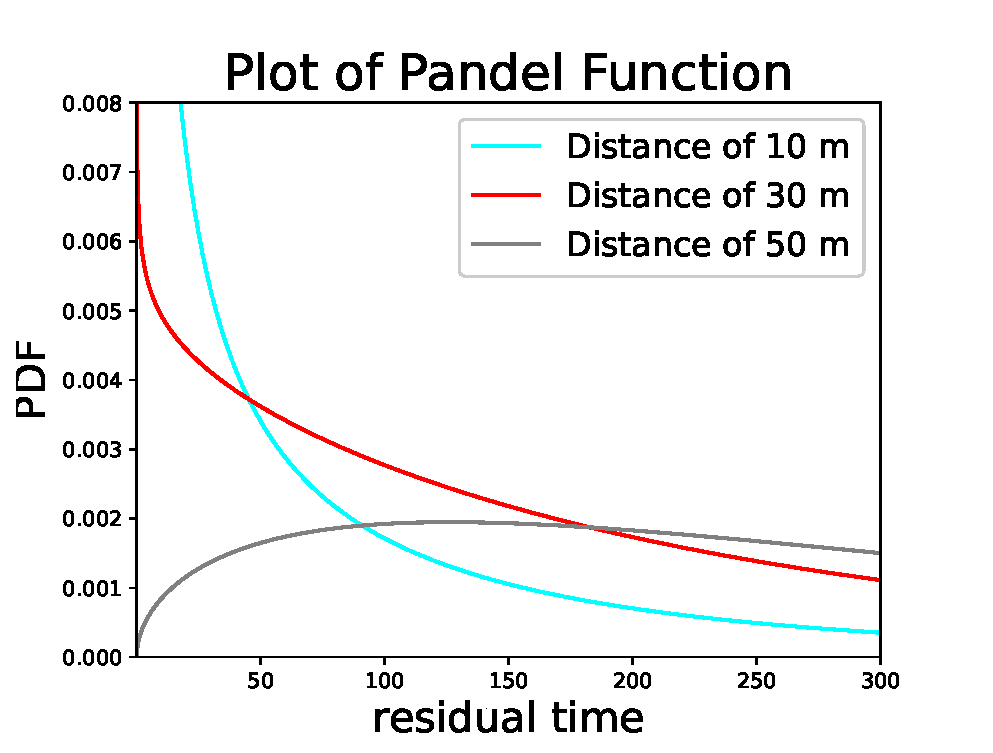
\includegraphics[width=12cm]{./Figures/pandel_plot.eps}
  \caption{A figure showing a plot of the pandel function over 300 nanoseconds with 10 meters, 30 meters and 50 meters of travel distances for the emitted light. }
  \label{fig:pandel}
\end{figure}
